\documentclass[preprint,prd,showpacs]{revtex4-1}
\usepackage{graphicx}

\newcommand{\pt}{\ensuremath{p_T}}
\newcommand{\met}{\ensuremath{E_{T}^{miss}}}
\newcommand{\gev}{~\mathrm{GeV}}
\newcommand{\tev}{~\mathrm{TeV}}
\newcommand{\ifb}{~\mathrm{fb}^{-1}}
\newcommand{\khz}{~\mathrm{KHz}}
\newcommand{\kt}{k_{T}}
\newcommand{\et}{E_{T}}

\newcommand{\trimmedgraphic}[2][]{
  \includegraphics[width=0.4\textwidth,trim={0.5cm 1cm 1.5cm 1cm},clip,#1]{#2}
}


\begin{document}
\title{Commercial associative memory performance for applications in track-based triggers at the Large Hadron Collider}
\author{Jordan Webster}
\affiliation{Argonne National Laboratory}
\author{Jinlong Zhang}
\affiliation{Argonne National Laboratory}

\date{\today}
\begin{abstract}
  Dense track environments in $pp$ collisions at the Large Hadron Collider (LHC) motivate the use of triggers with dedicated hardware for fast track reconstruction. The ATLAS Collaboration is in the process of implementing a Fast Tracker (FTK) trigger upgrade, in which Content Addressable Memories (CAMs) will be used to rapidly match hit patterns with large banks of simulated tracks. The FTK CAMs are produced primarily at the University of Pisa. However, commercial CAM technology is developing at a fast pace for computer networking applications. This document contains proceedings for a poster presented on new studies comparing FTK CAMs to cutting edge ternary CAMs developed by Cavium. The comparison is intended to guide the design of future track-based trigger systems for the next Phase at the LHC.
\end{abstract}

\maketitle

\section{Introduction}\label{sec:Introduction}

The Large Hadron Collider (LHC) is designed to collide protons 40 million $pp$ times per second, which produces an enormous amount of data. Due to hardware limitations the ATLAS and CMS experiements are only capable writing approximately 100 collisions (or events) to disk per second. As a result, both experiments are forced to implement multi-level trigger systems designed to rapidly identify events with interesting physics. Events that are not flagged in these trigger systems are discarded on the fly so that the event rate is reduced before data is saved to disk.

Reconstructing charged particle tracks in silicon detector layers is critical for making trigger decisions because tracks are often associated with interesting objects like electrons, muons, and $b$-jets. Tracks can also be used to estimate missing transverse energy and to identify primary vertices. Unfortunately, track reconstruction is computationally expensive. Typical collisions contain thousands of silicon detector hits and hundeds of tracks with transverse momentum above $1\gev$. Performing a full helical fit of every single combination of hits in the silicon detector layers is impossible even at a $100\khz$ event rate. The solution is to build dedicated hardware like the Fast Track Trigger (FTK) system for ATLAS~\cite{Shochet:1552953}, which can do approximate track reconstruction at $100\khz$.

A key component of all hardware-based track triggers (FTK included) is Associative Memory (AM), or Content Addressable Memory (CAM). CAMs are a special type of computer memory used for high speed search applications. They are built for the general task of comparing input data against a table of stored data to look for matches. The CAMs used for FTK are loaded with large banks of precomputed hit patterns that are associated with simulated tracks. When hits from the silicon detector readout system are passed into FTK the CAMs return a list of matched hit patterns. Each matched pattern (or \textit{road}) therefore represents a possible track, and the hit values can be used to compute helix parameters and a $\chi^{2}$ value.

Figure~\ref{fig:am_cartoon} shows a drastically simplified cartoon model of a CAM. The memory is composed of a strucured lattice of comparators. Hits arriving from the left are compared with precomputed hit patterns, represented by vertical strings of characters. A pattern fires if there is a matching hit in each detector layer. Additional logic can be used to allow patterns to fire when they have missing hits in one or more layers due to detector innefficiency.

\begin{figure*}[!htb]
\begin{center}
\includegraphics[width=0.4\textwidth,trim={7cm 6cm 7cm 6cm},clip]{figures/am_cartoon}
\caption{Simplified cartoon of a CAM used for a identifying track candidates using 5 silicon detector layers. The cartoon shows 8 pre-stored hit patterns. Each pattern has one character (representing one hit coordinate) per layer. Hits enter the CAM on the left side of the cartoon. Matches are triggered if a pattern has a matching hit in each layer.}
\label{fig:am_cartoon}
\end{center}
\end{figure*}

%For example, consider the cartoon 5-layer detector shown in Figure~\ref{

%For a simple example consider Figure~\ref{fig:pattern_cartoon}, which shows a two-dimensional cartoon schematic of 5 silicon detector layers with multiple hits represented by red stars. The layers are boxed off into small ganged pixel regions (referred to as \textit{super strips} in FTK). Patterns are loaded in a CAM

%\begin{figure*}[!htb]
%\begin{center}
%\includegraphics[width=0.4\textwidth]{figures/pattern_cartoon}
%\caption{Cartoon showing an example track-like pattern in X detector layers...}
%\label{fig:pattern_cartoon}
%\end{center}
%\end{figure*}




\section{Test Setup}\label{sec:TestSetup}

Cavium is commercial developer of AM technology. A test setup was constructed at Argonne National Lab to measure the performance of a cutting edge Cavium AM chip and determine if it could replace dedicated AMs in future LHC track triggers.
A “ternary” CAM (tCAM) was used for these tests. This allowed for the use of hit patterns “don’t care” (DC) bits, as is done in FTK. Tests were done using 128 bit FTK-like patterns, varying the number of DC bits per pattern between 0 and 16.

\subsection{Hardware}

A 22-core Network Processor (OCTEON CN6800) is connected to a Neuron Search Processor Board, or NSP (CNSP1600).
The NSP contains a tCAM chip with 4 memory clusters. 
Communication to the Network Processor is established through a serial console.

\begin{figure*}[!htb]
\begin{center}
\includegraphics[width=0.8\textwidth]{figures/TCAM_pic}
\caption{Photograph of the board...}
\label{fig:board_pic}
\end{center}
\end{figure*}

\subsection{Software}

FIXME



\section{Results}\label{sec:Results}

The Cavium tCAM can store 235K FTK-like patterns with no DC bits [left] and perform roughly 24M lookups per second [right].

For comparison, the FTK AM stores 128K patterns and runs at 100 MHz.

\begin{figure*}[!htb]
\begin{center}
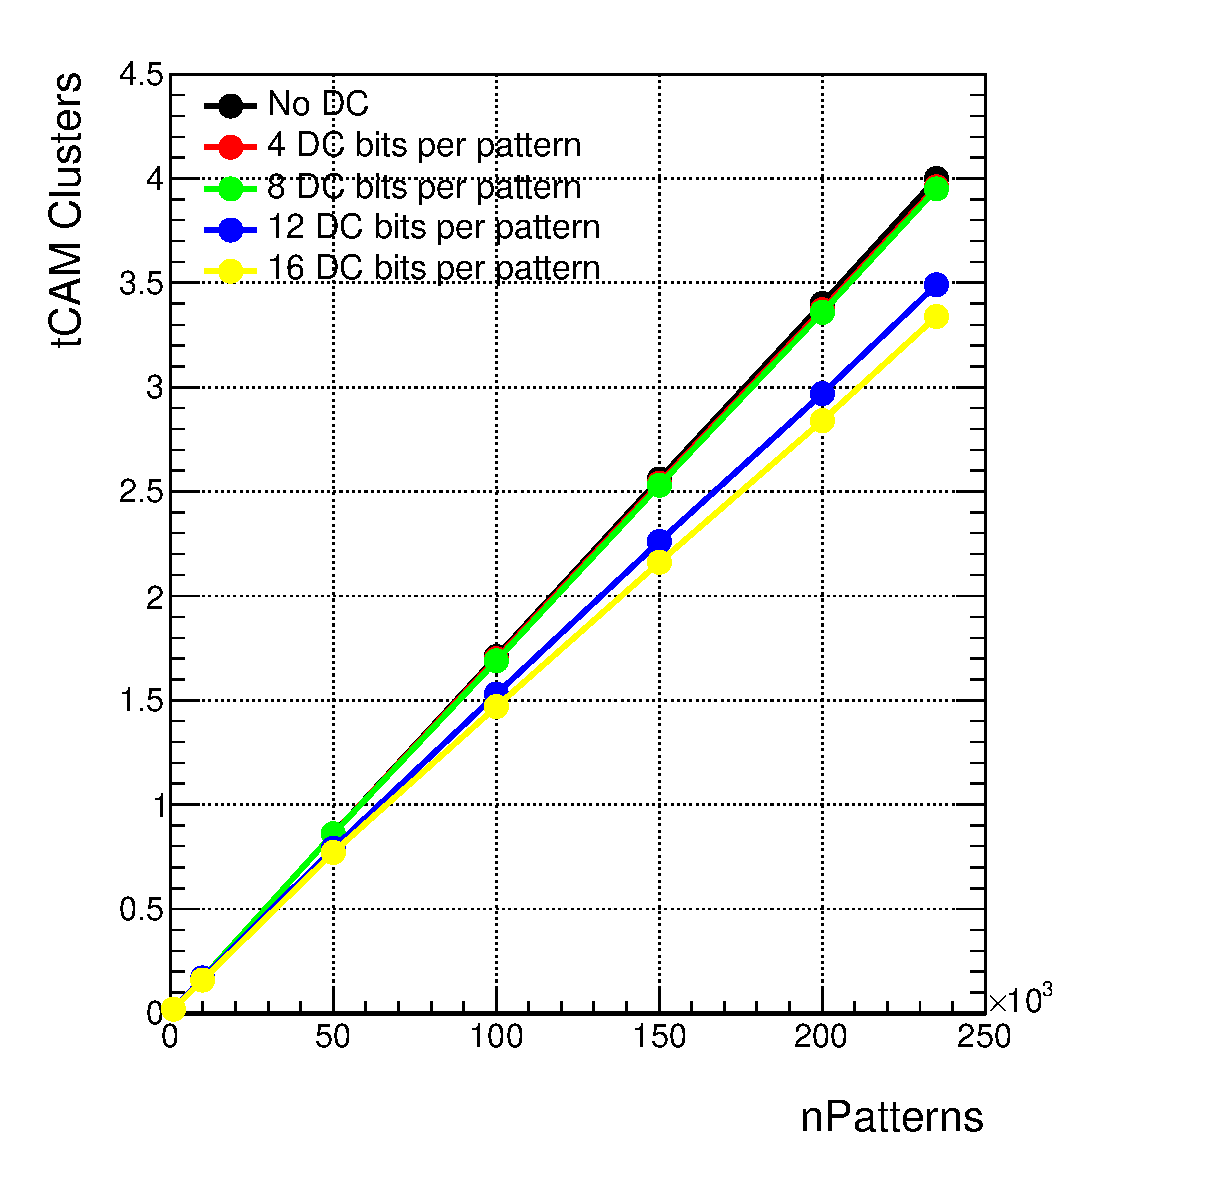
\includegraphics[width=0.45\textwidth]{figures/PlotTcamData_eps/001}
%\hspace{1cm}
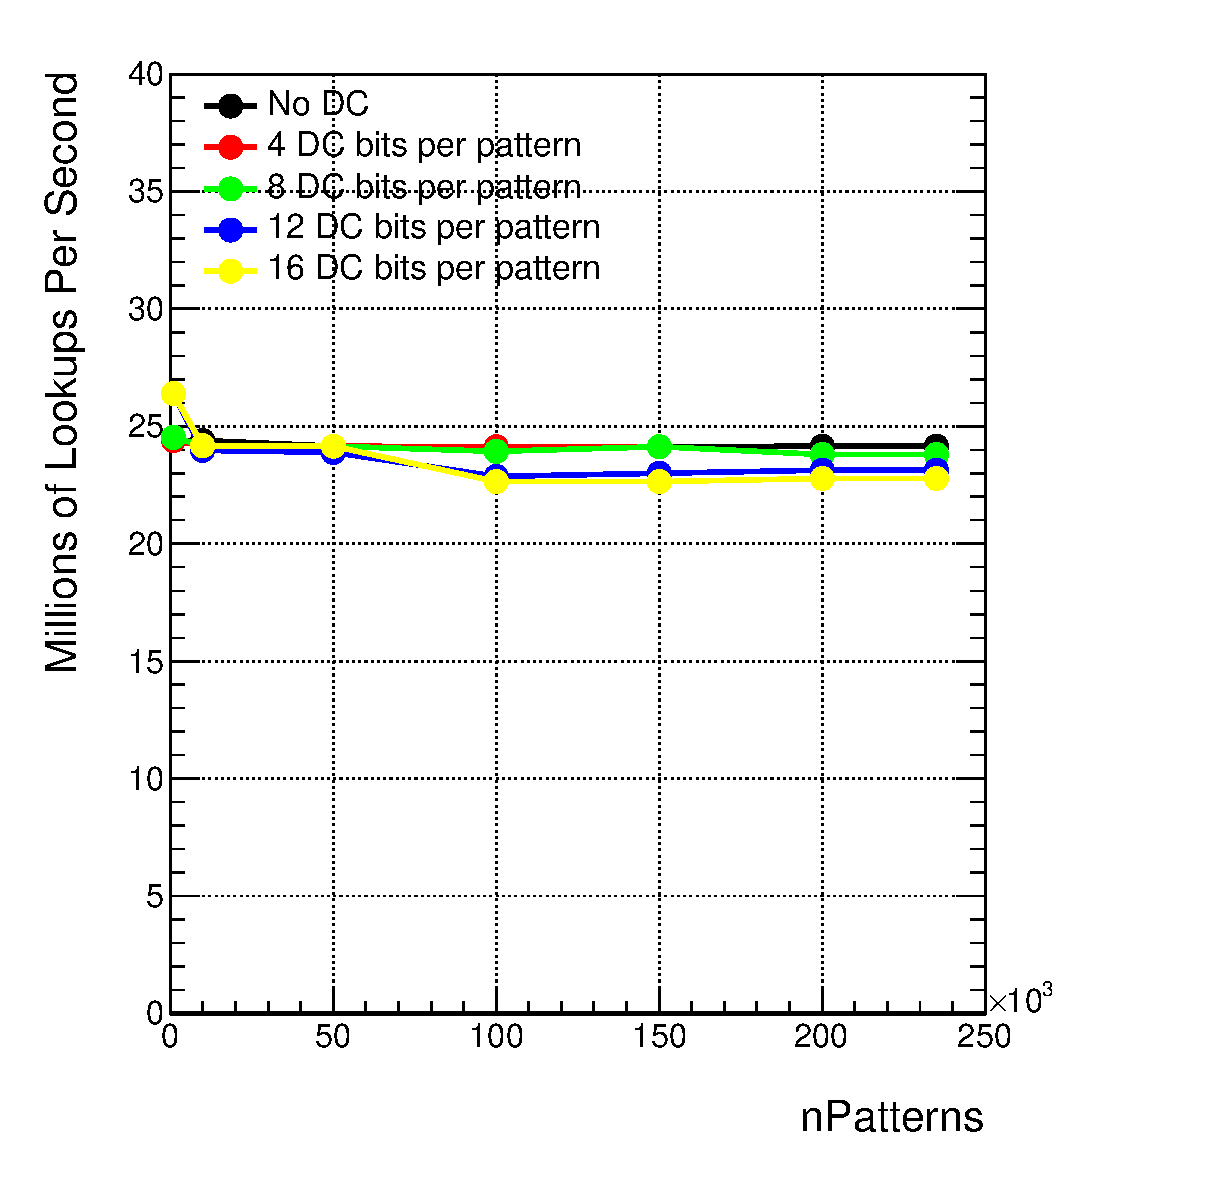
\includegraphics[width=0.45\textwidth]{figures/PlotTcamData_eps/002}
\caption{FILLME}
\label{fig:nsp_perf_plots}
\end{center}
\end{figure*}


\section{Discussion}\label{sec:Discussion}

Results indicate that commercial tCAMs from Cavium have sufficient storage capacity, but are only fast enough to perform FTK-like track reconstruction at a ~25 KHz event rate. Furthermore, Cavium's chips are  roughly 20× more expensive than the latest FTK AM chips (excluding R\&D costs). However, since the cost of commercial technology drops faster than the cost of dedicated hardware, the commercial options are likely to become more promising in the near future.

\section{Acknowledgments}
This work was supported by the U.S. Department of Energy, Office of Science under contract DE-AC02-06CH11357.

\bibliography{proc}

\end{document}




